\section{How Many Deltahedron Exist?}
\label{sec:deltahedron}

In this section, we share a proof due to
Fushsida-Hardy \cite{deltahedron} that there are
only eight deltahedron.

A \EMPH{deltahedron} is a polyhedron whose
faces are all equilateral triangles. Two examples are shown
in \figref{deltahedron}.


\begin{figure}[htb]
\centering
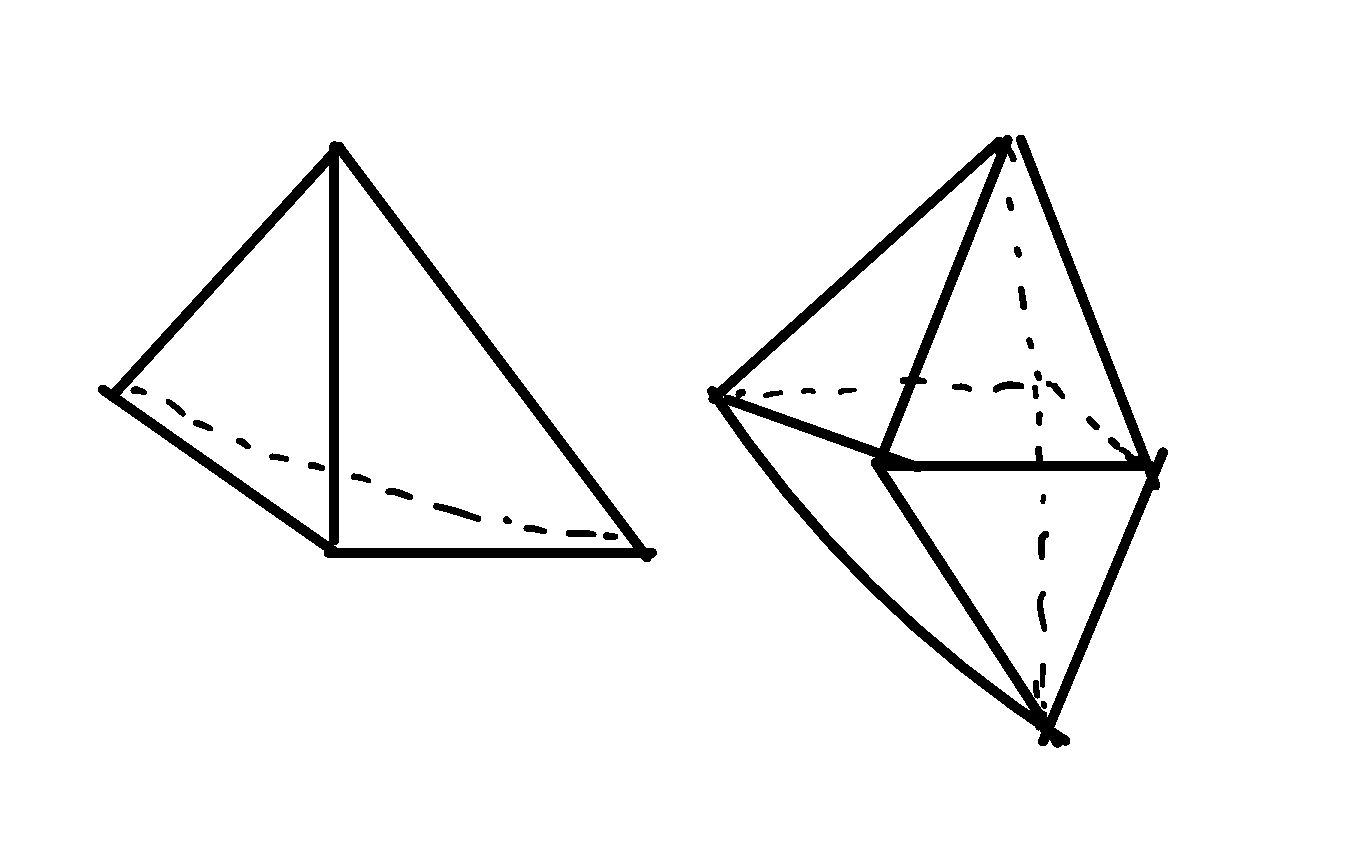
\includegraphics[width=.3\textwidth]{curvature/deltahedron}
\caption{Two deltahedron. A tetrahedron and an octahedron.}
\label{fig:deltahedron}
\end{figure}

How many convex deltahedron are there?
Any convex deltahedron is homeomorphic to the sphere.
So we know $\chi(S)=2$ and there is no boundary.

Let $T=(V,E,F)$  be a triangulation of the sphere.
Here, after scaling by $\pi$ the curvature of a vertex
is $k(v)=4-deg(v).$
Then, the Gauss-Bonnet theorem
states,

$$\sum_{v\in V}K(v)=2\cdot  3\cdot 2.$$
Since we have a triangulation each
vertex must have degree at lease three.
Thus, $k(v)\leq 3$ for all $v$. But, since we have
convex faces, $k(v)\geq 1$ for all $v$.

So, for $1\leq k(v_i)\leq 3$ and  $\sum k(v_i)=12$,
so we only need to examine a finite number (19) of cases.
For example, if the curvature at each vertex is three then,
we have four vertices. Each vertex is incident to three edges
and each edge has two vertices so $\frac{3}{2}4=E=6$ and
there are four faces. This is the tetrahedra.




